\begin{frame}{terminology: packers}
    \begin{itemize}
    \item programs that decode and run code at runtime called \textit{packers}
    \item packers exist to do this for non-malware reasons
    \item example motivations:
        \begin{itemize}
        \item compression
        \item packaging libraries + executable together
        \end{itemize}
    \end{itemize}
\end{frame}

\begin{frame}{from UPX documentation}
\pdftooltip{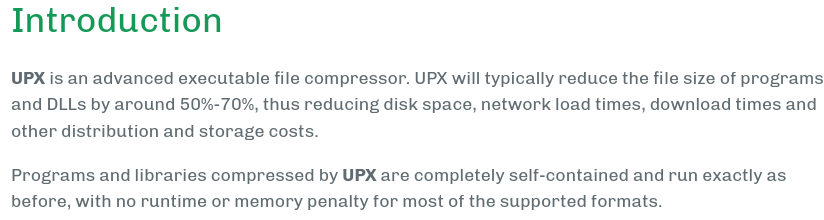
\includegraphics[width=\textwidth]{../antianti/upx-intro}}{
UPX is an advanced executable file compressor. UPX will typically reduce the file size of programs and DLLs by around 50\%-70\%, thus reducing disk space, network load times, download times and other distribution and storage costs.\textLF\textLF%
Programs and libraries compressed by UPX are completely self-contained and run exactly as before, with no runtime or memory penalty for most of the supported formats.
}
\vspace{0.5cm}
\hrule
\vspace{0.5cm}
\pdftooltip{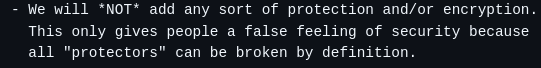
\includegraphics[width=\textwidth]{../antianti/upx-not-prot}}{
We will *NOT* add any sort of protection and/or encryption. This only gives people a false feeling of security because all "protectors" can be broken by definition.%
}
\end{frame}


